\documentclass{cssheet}

%--------------------------------------------------------------------------------------------------------------
% Basic meta data
%--------------------------------------------------------------------------------------------------------------

\title{Symmetriegruppen bei Fliesen}
\author{Prof. Dr. Christian Spannagel}
\date{\today}
\hypersetup{%
    pdfauthor={\theauthor},%
    pdftitle={\thetitle},% 
    pdfsubject={Aufgabenblatt Algebra},%
    pdfkeywords={algebra}
}

%--------------------------------------------------------------------------------------------------------------
% document
%--------------------------------------------------------------------------------------------------------------

\begin{document}
\printtitle


\textbf{Aufgabe 1 (Fliesen):} 

Um welche Symmetriegruppen handelt es sich bei den folgenden Fliesen? Analysiert die Fliesen und vergleicht sie mit den Symmetriegruppen von geometrischen Figuren, die ihr bereits kennt.

\begin{figure}[H]
	\centering
	\setlength{\tabcolsep}{6pt} % horizontaler Abstand zwischen Spalten
	\renewcommand{\arraystretch}{1.2} % vertikaler Abstand zwischen Zeilen (auch für Text über Bild)
	\begin{tabular}{ccccc}
		\textbf{Fliese Nr. 1} & \textbf{Fliese Nr. 2} & \textbf{Fliese Nr. 3} & \textbf{Fliese Nr. 4} & \textbf{Fliese Nr. 5} \\
		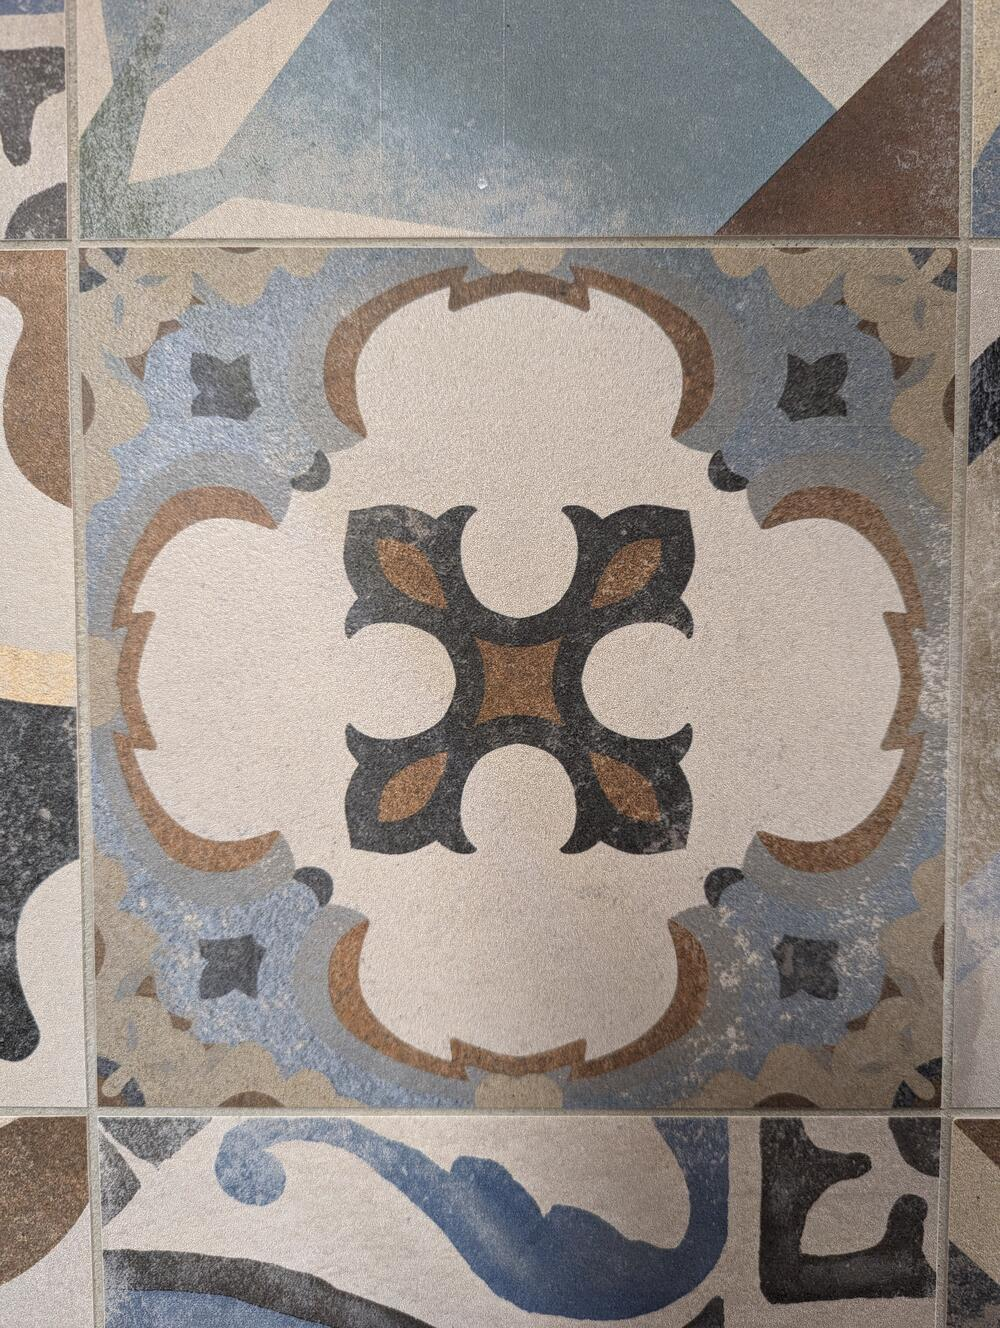
\includegraphics[height=4cm]{fliesen/fliese01.jpg} &
		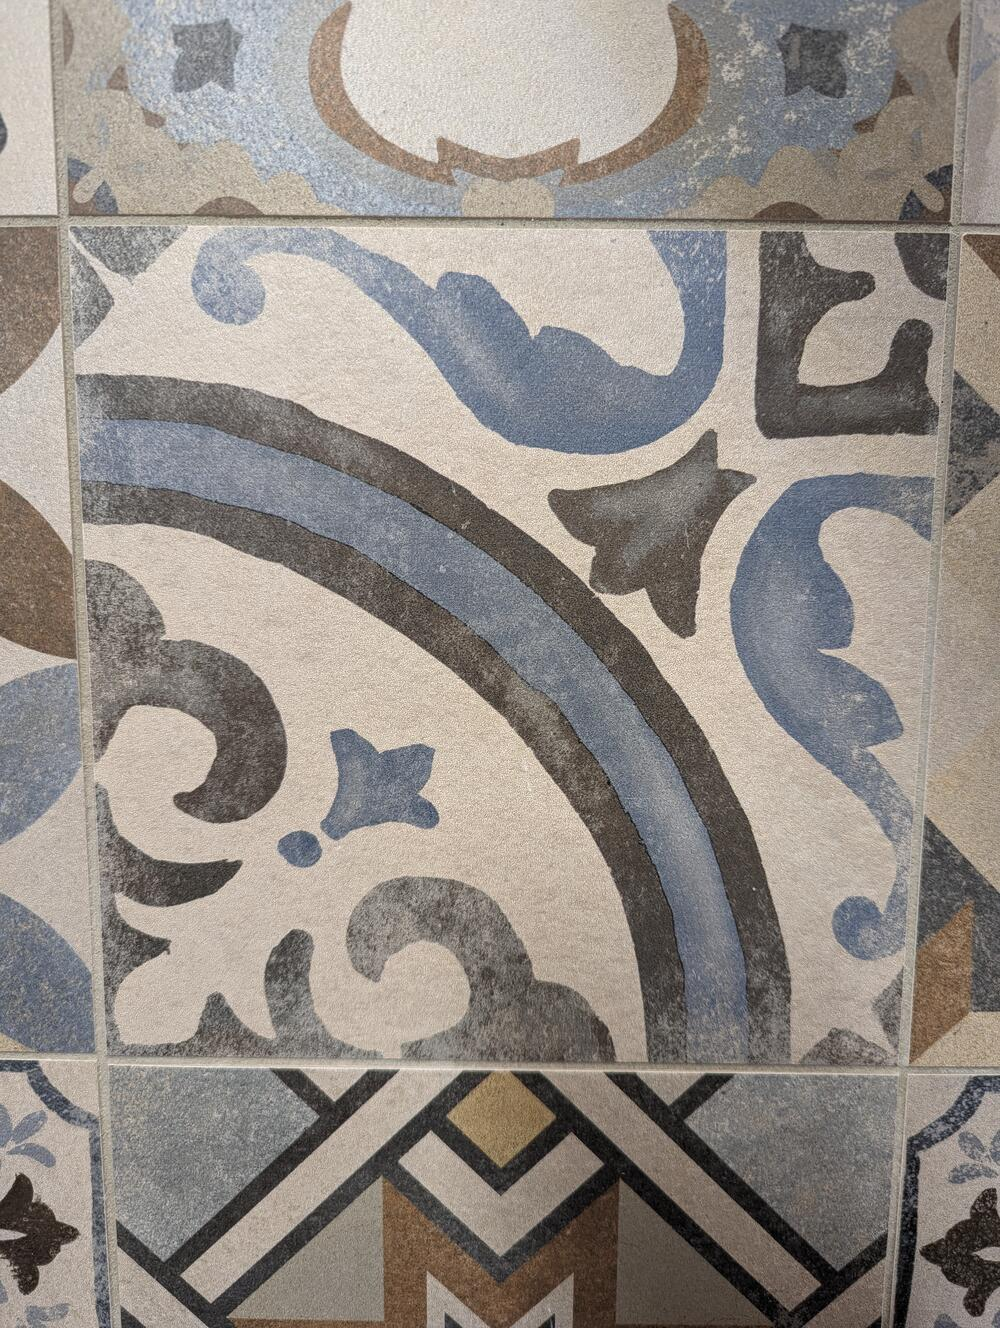
\includegraphics[height=4cm]{fliesen/fliese02.jpg} &
		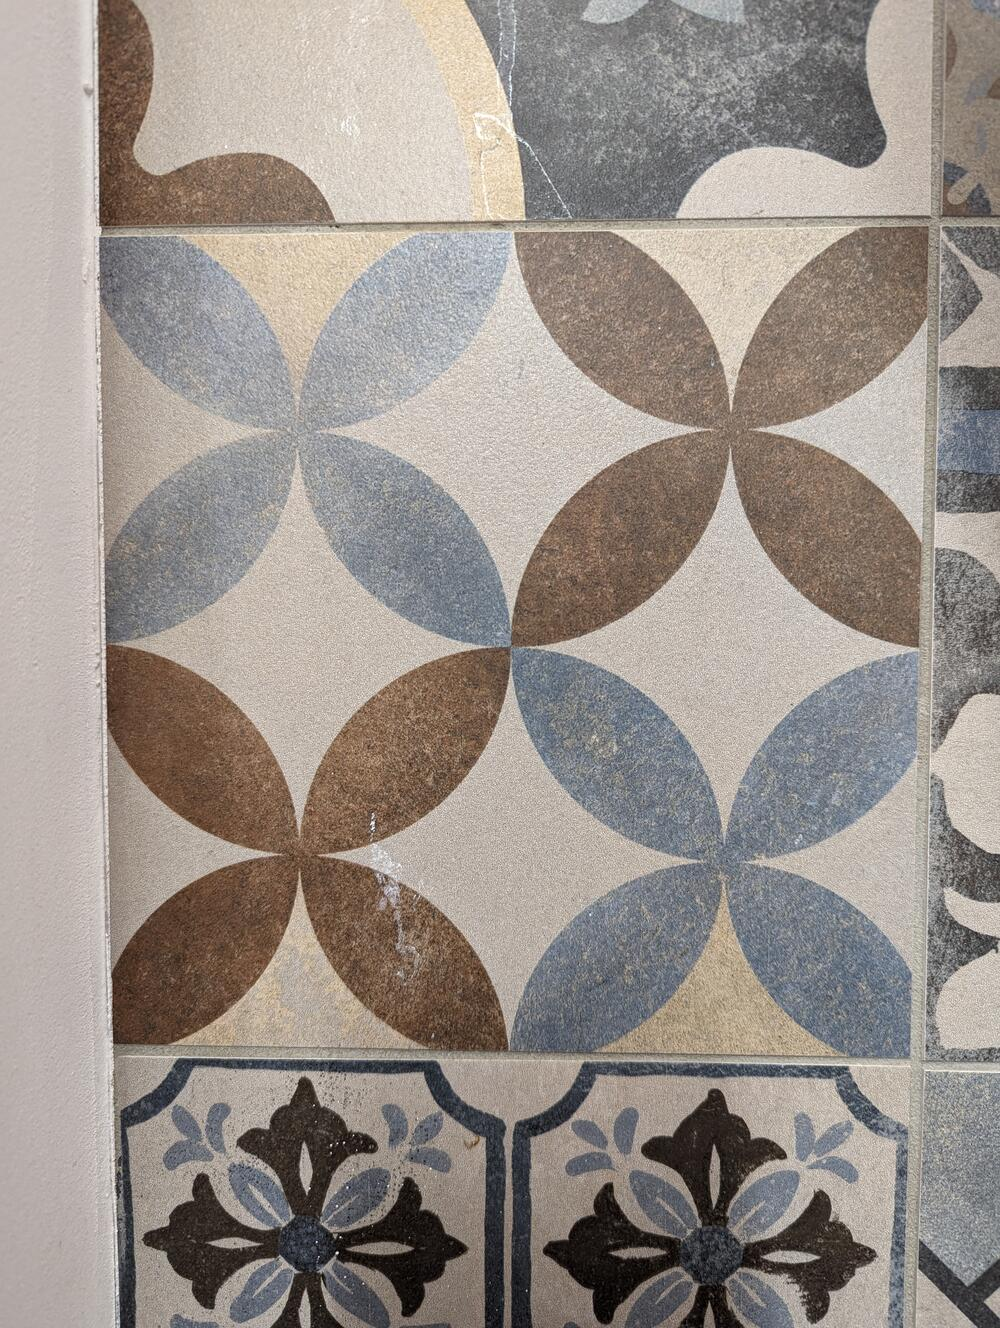
\includegraphics[height=4cm]{fliesen/fliese03.jpg} &
		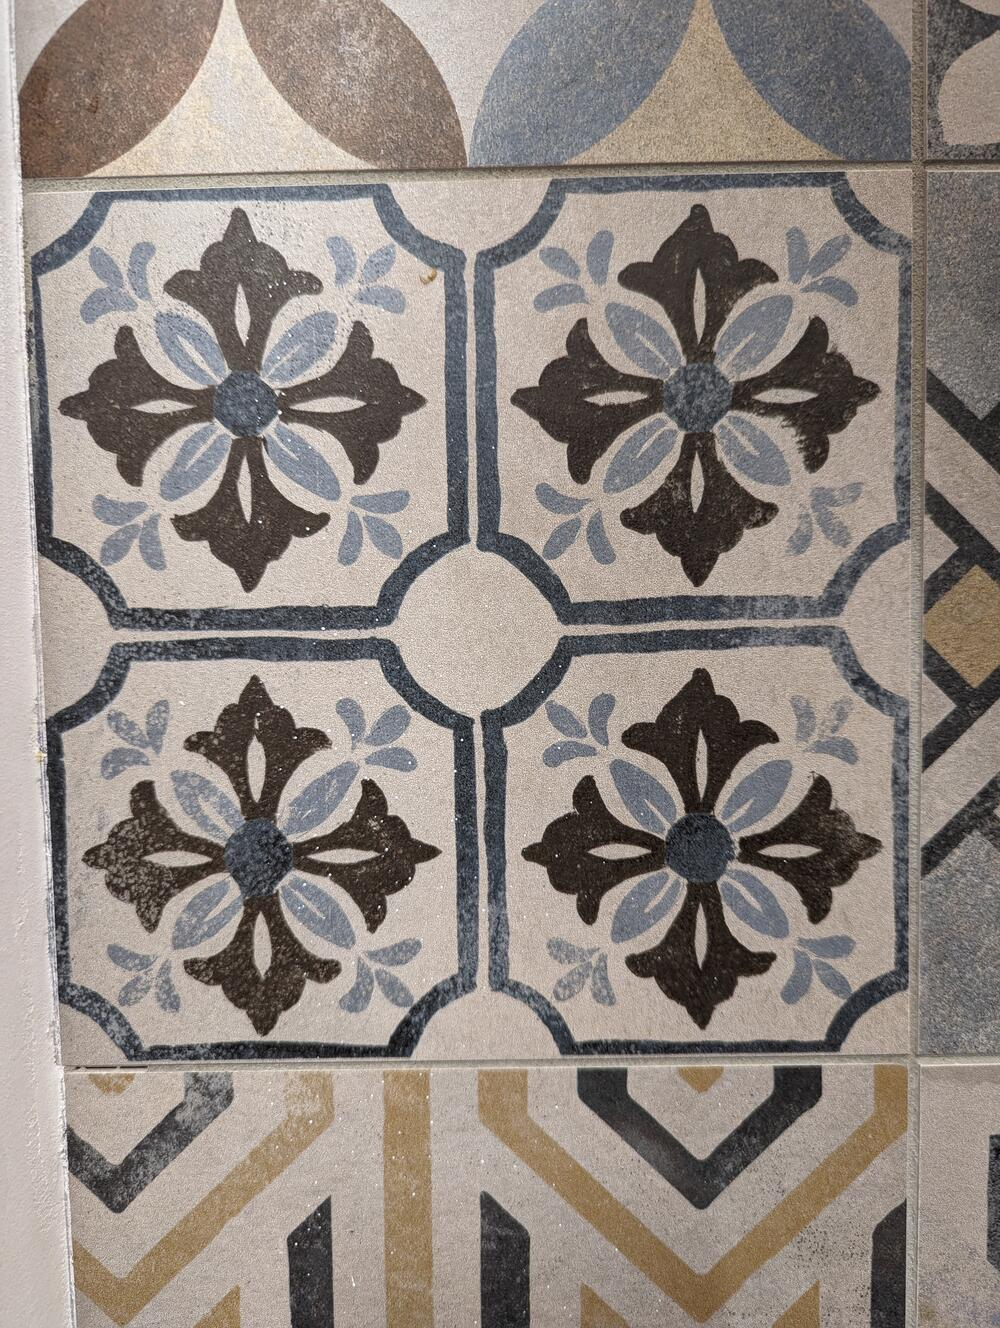
\includegraphics[height=4cm]{fliesen/fliese04.jpg} &
		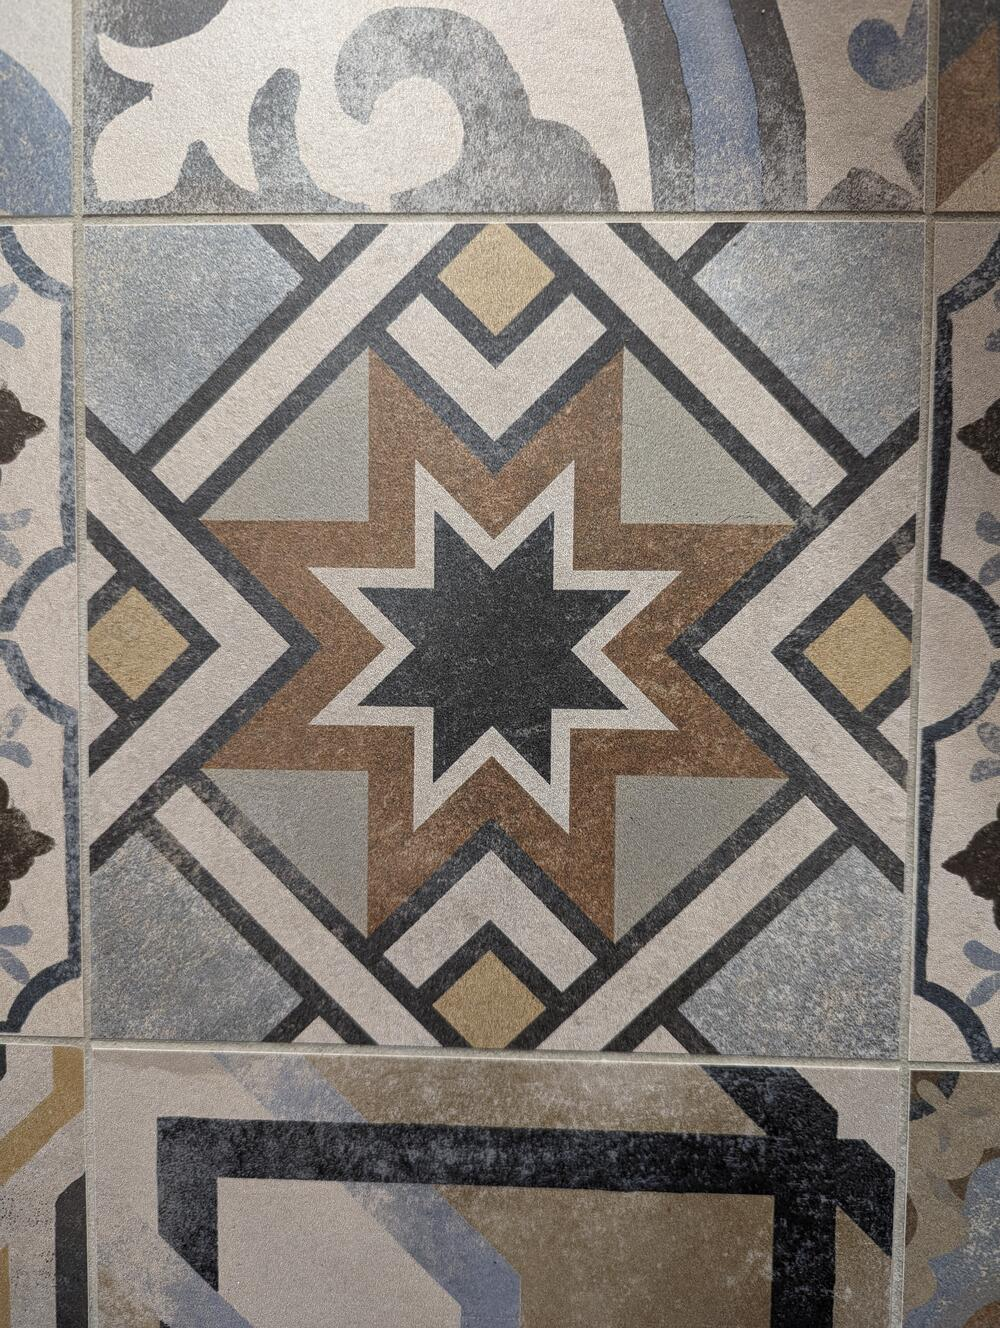
\includegraphics[height=4cm]{fliesen/fliese05.jpg} \\
		\textbf{Fliese Nr. 6} & \textbf{Fliese Nr. 7} & \textbf{Fliese Nr. 8} & \textbf{Fliese Nr. 9} & \textbf{Fliese Nr. 10} \\
		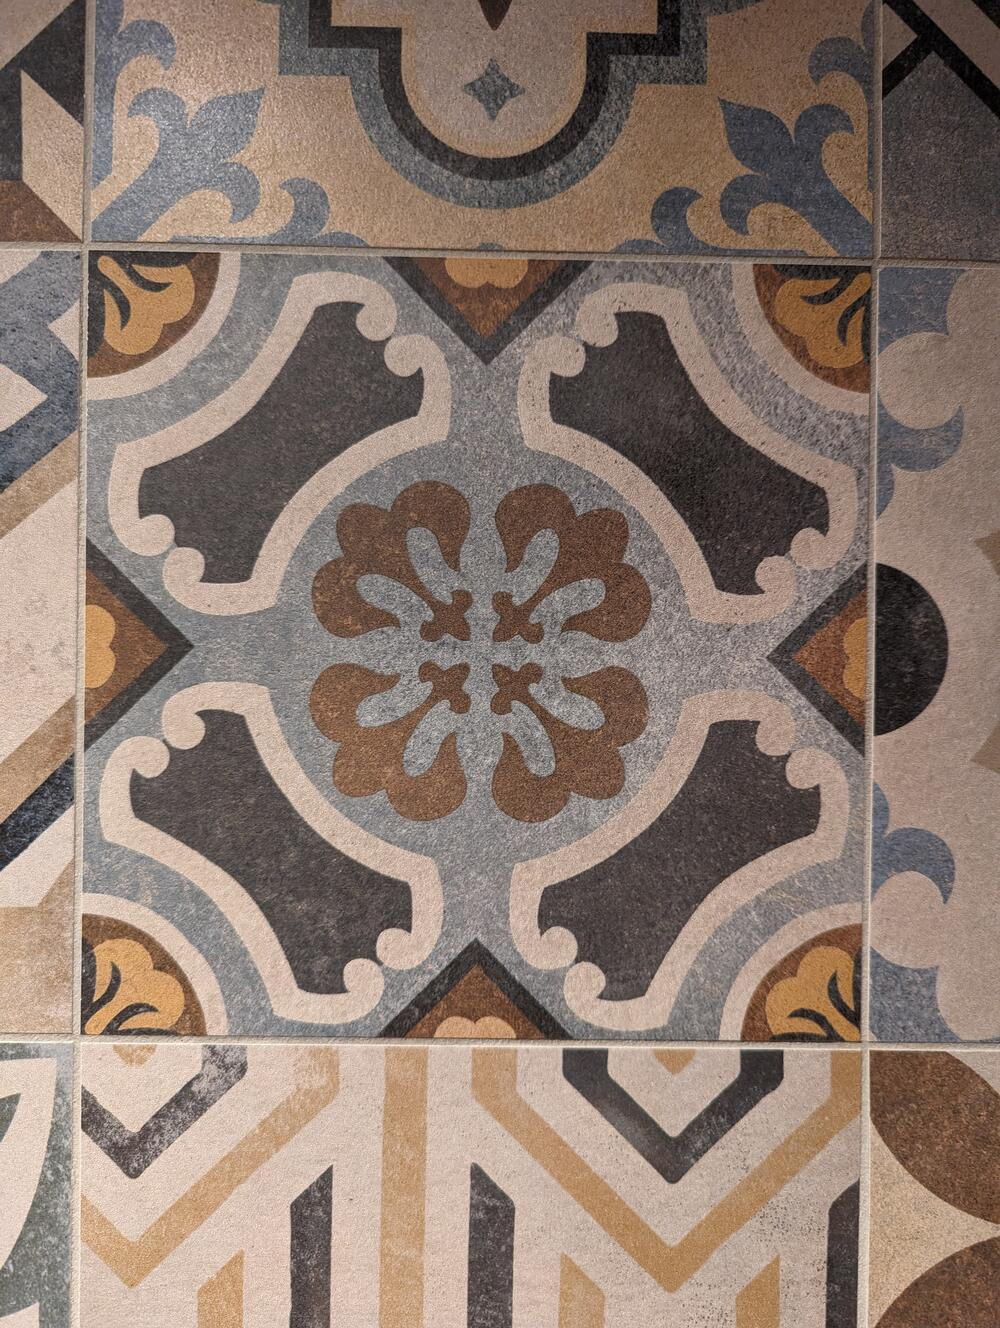
\includegraphics[height=4cm]{fliesen/fliese06.jpg} &
		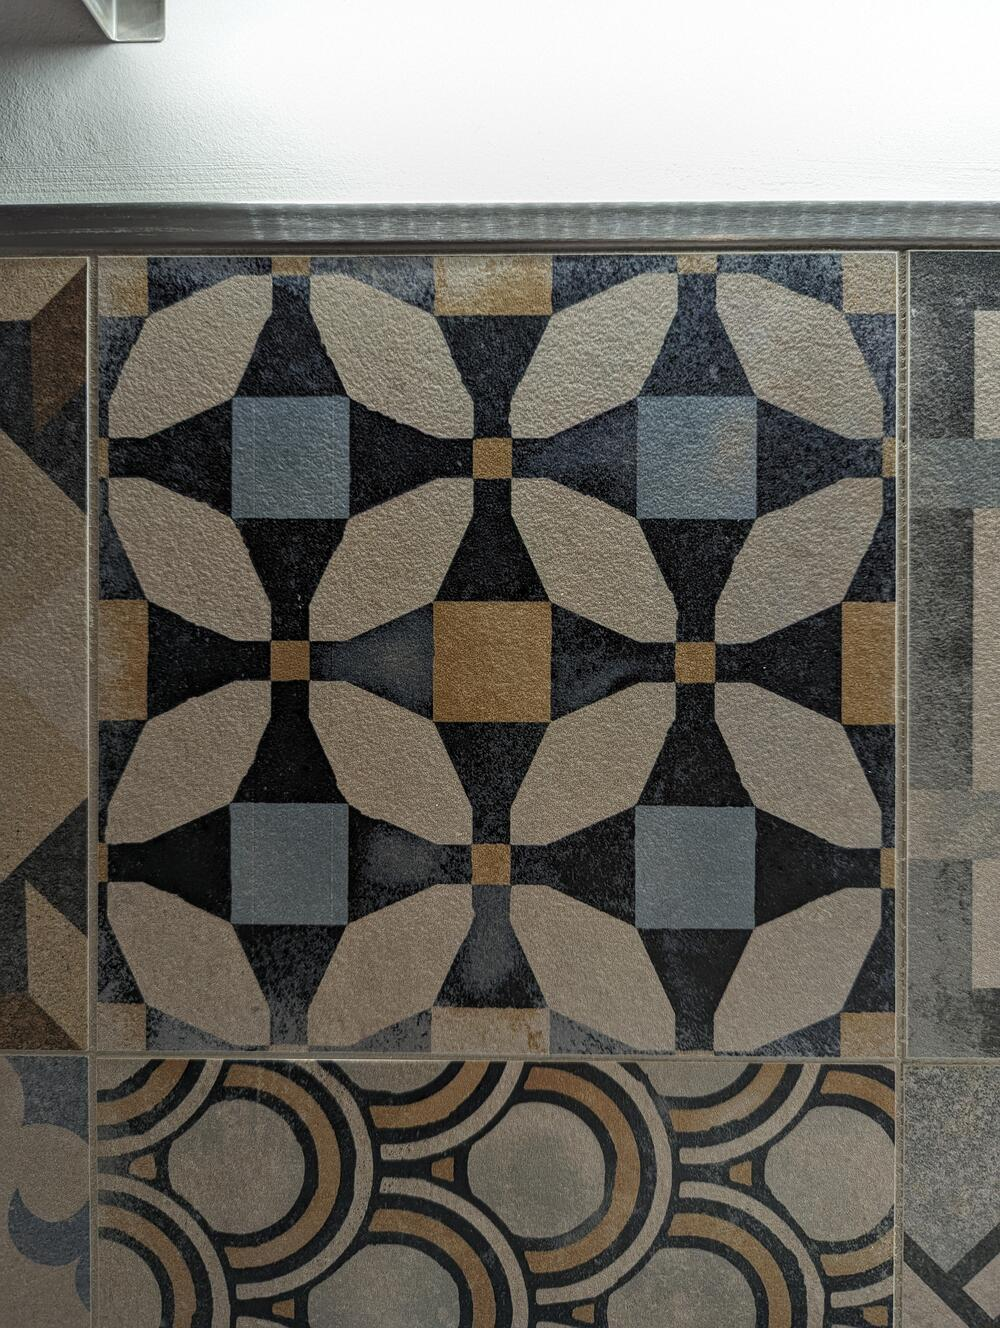
\includegraphics[height=4cm]{fliesen/fliese07.jpg} &
		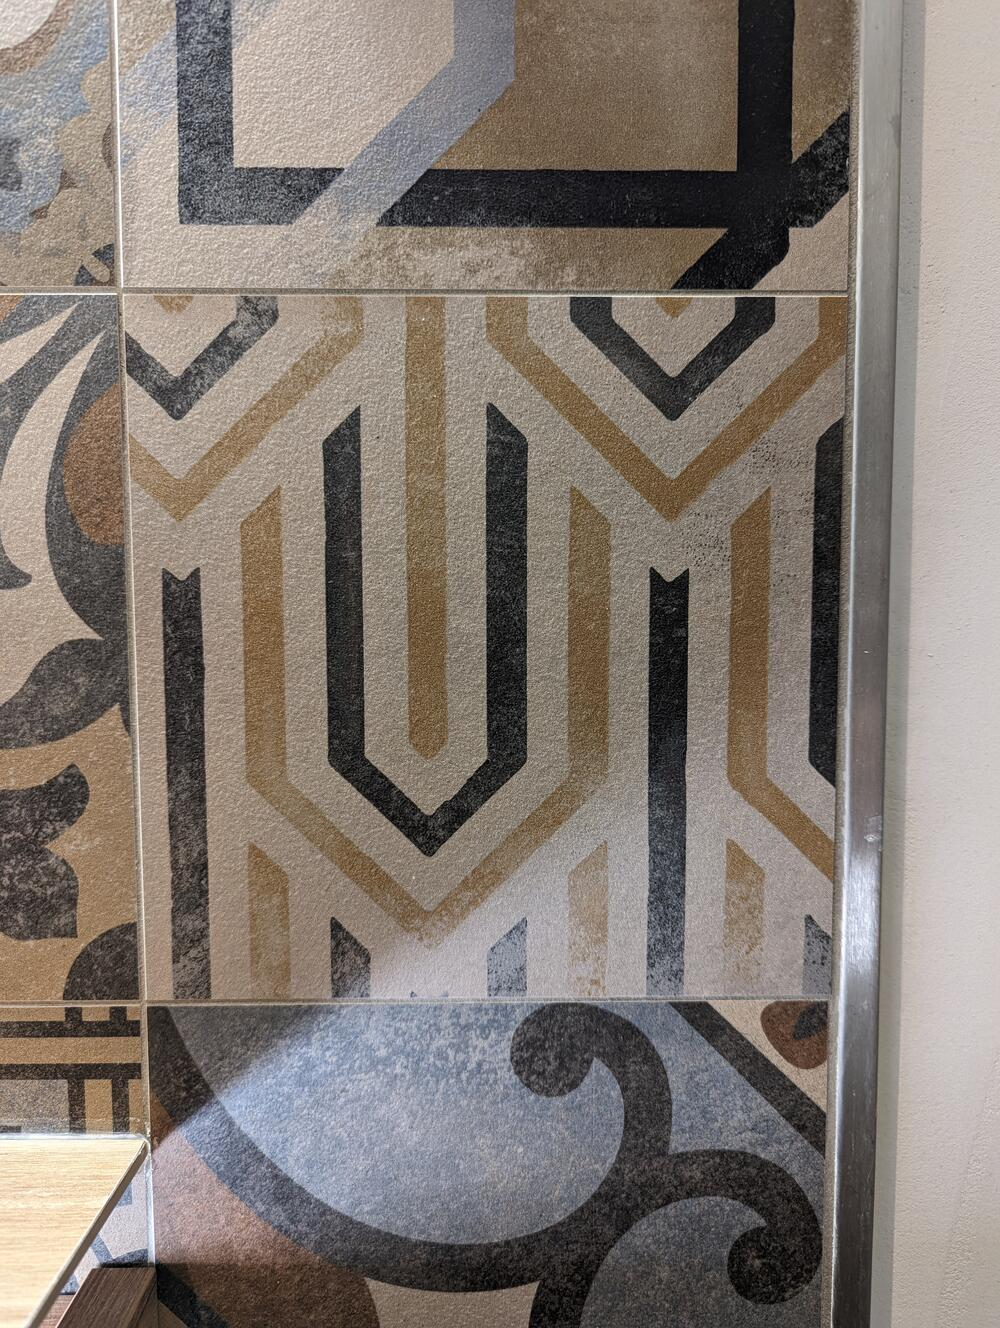
\includegraphics[height=4cm]{fliesen/fliese08.jpg} &
		
\includegraphics[height=4cm]{fliesen/fliese09.jpg} &
		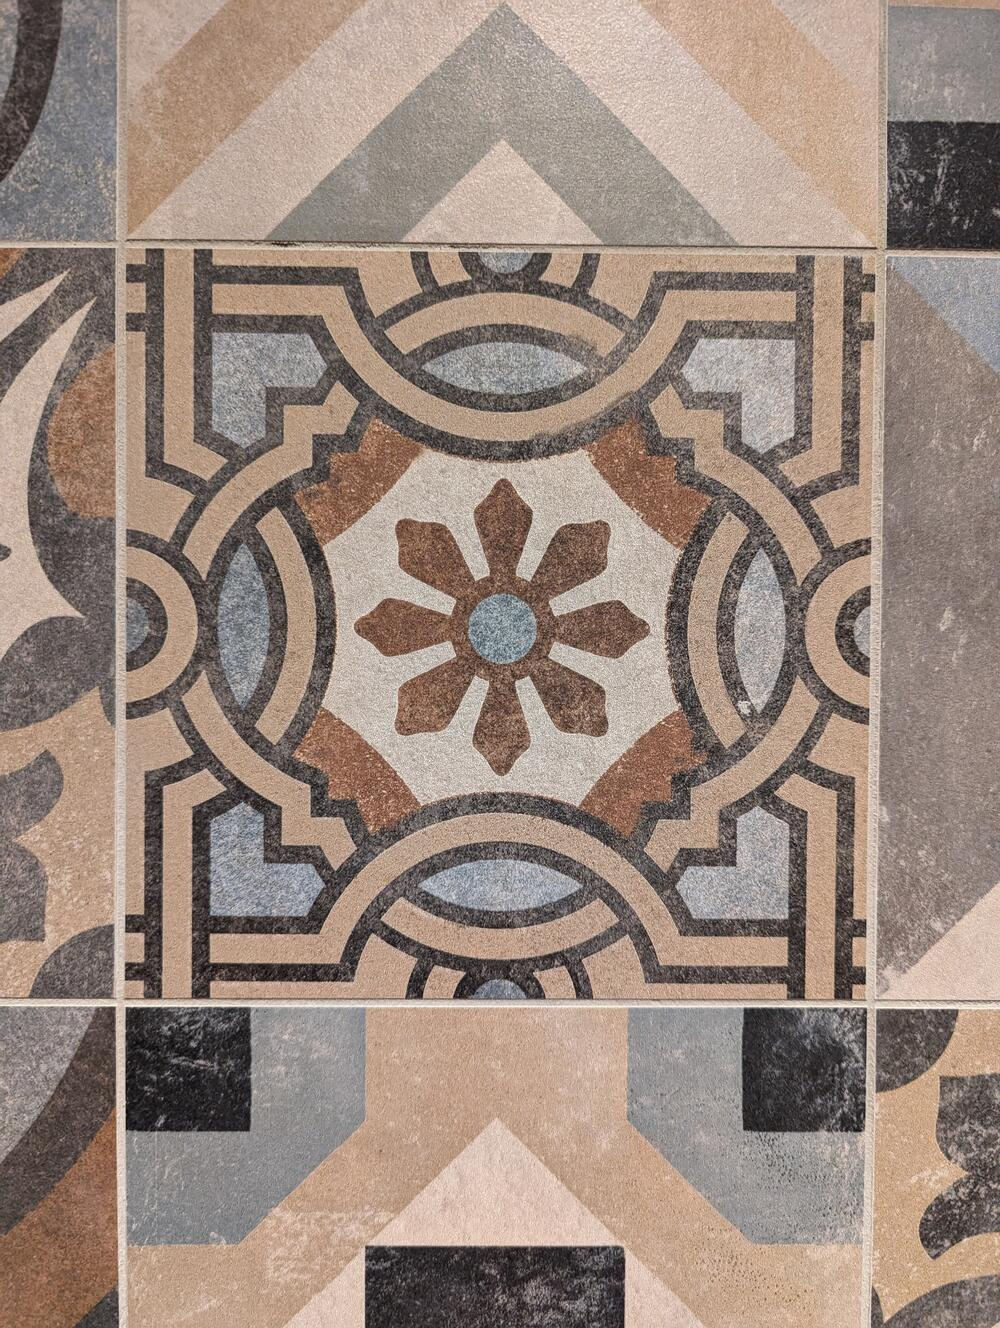
\includegraphics[height=4cm]{fliesen/fliese10.jpg} \\
		\textbf{Fliese Nr. 11} & \textbf{Fliese Nr. 12} & \textbf{Fliese Nr. 13} & \textbf{Fliese Nr. 14} & \textbf{Fliese Nr. 15} \\
		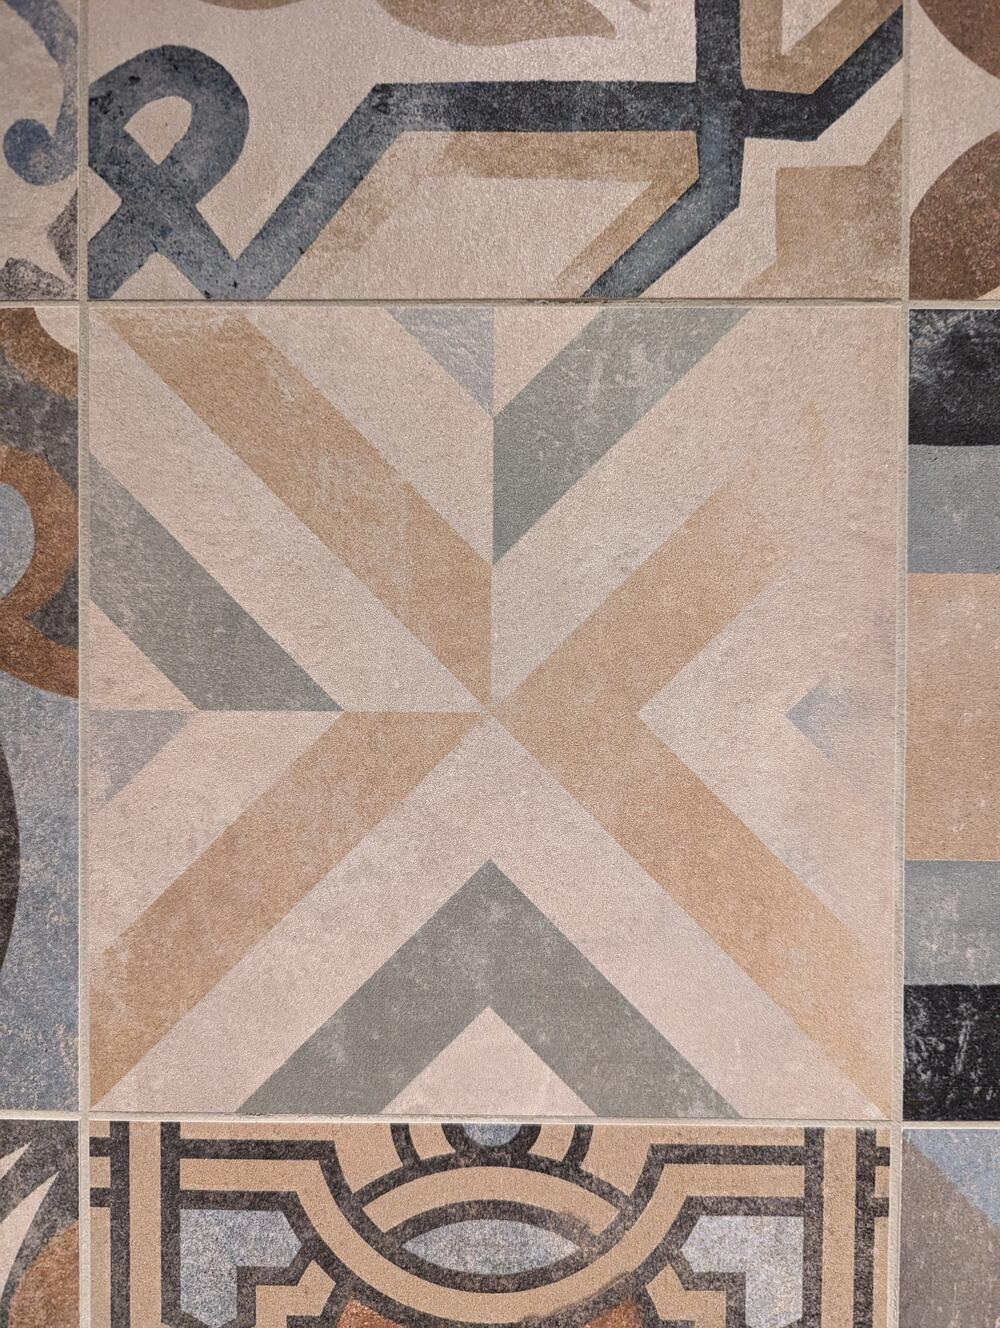
\includegraphics[height=4cm]{fliesen/fliese11.jpg} &
		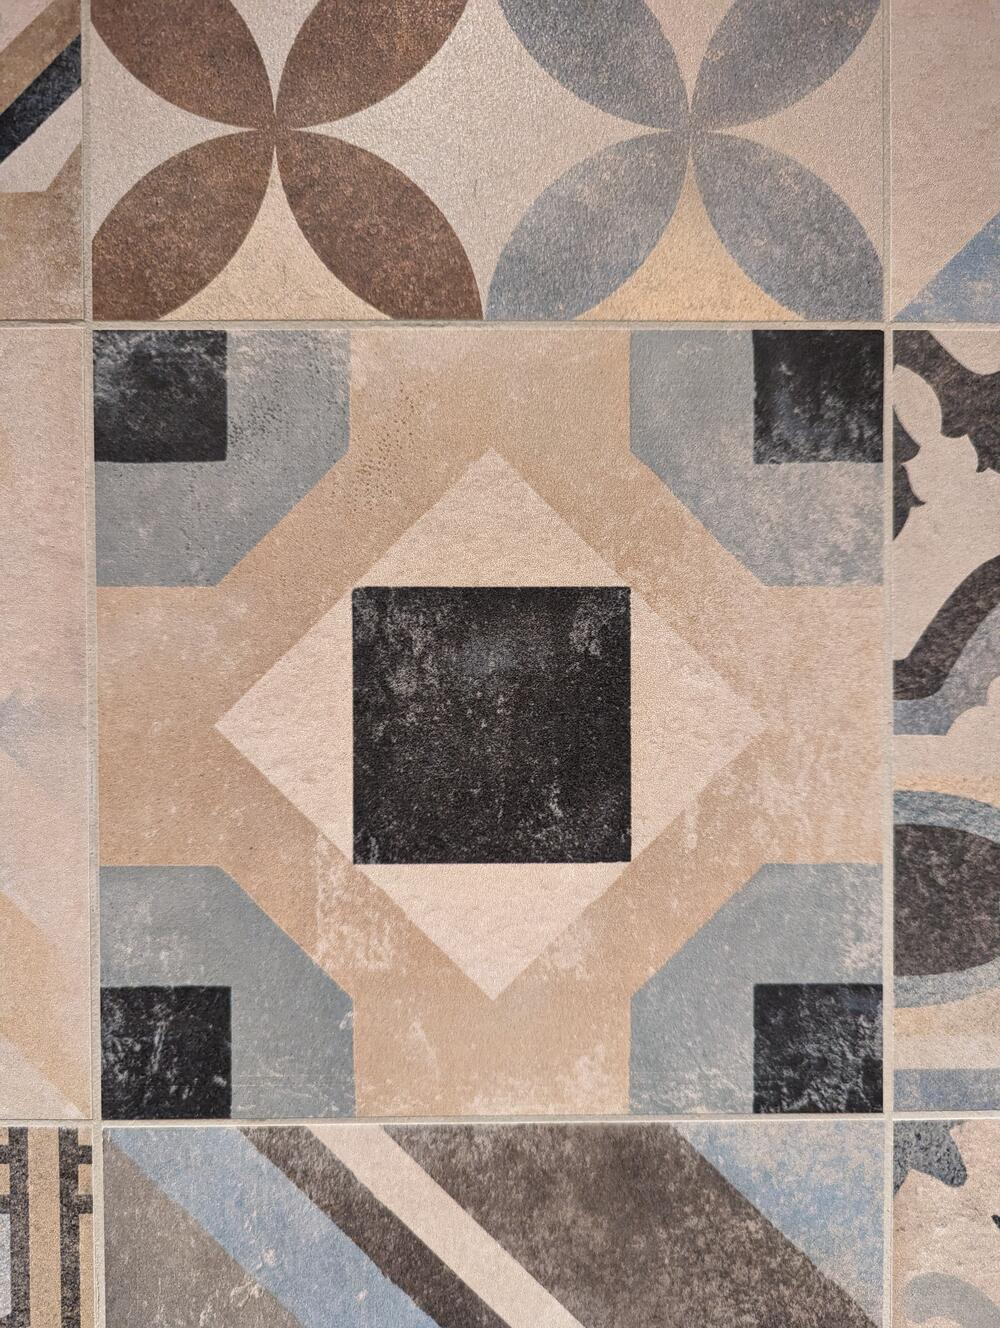
\includegraphics[height=4cm]{fliesen/fliese12.jpg} &
		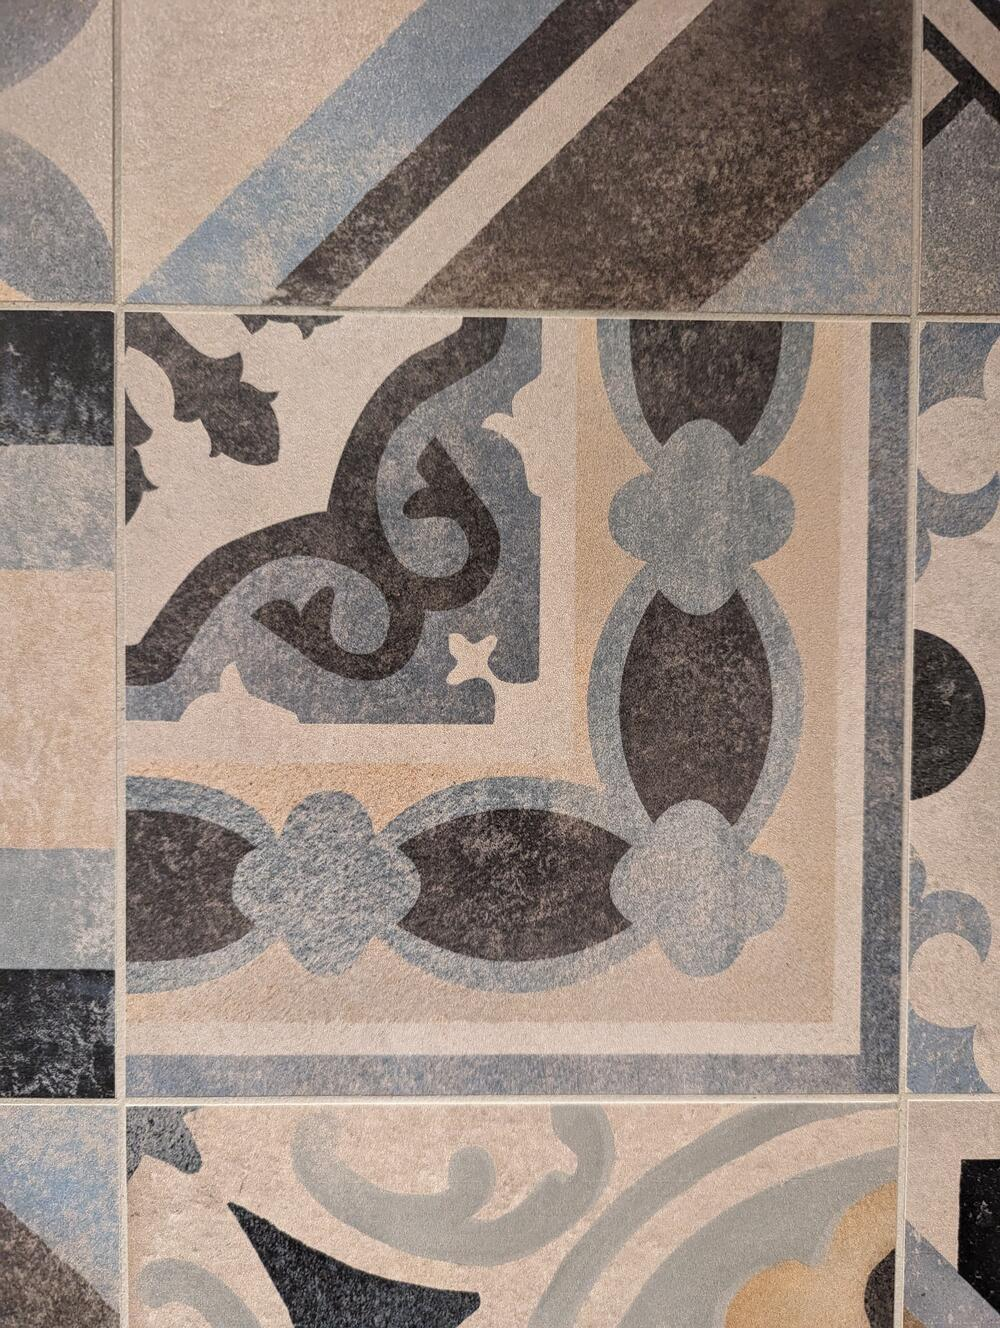
\includegraphics[height=4cm]{fliesen/fliese13.jpg} &
		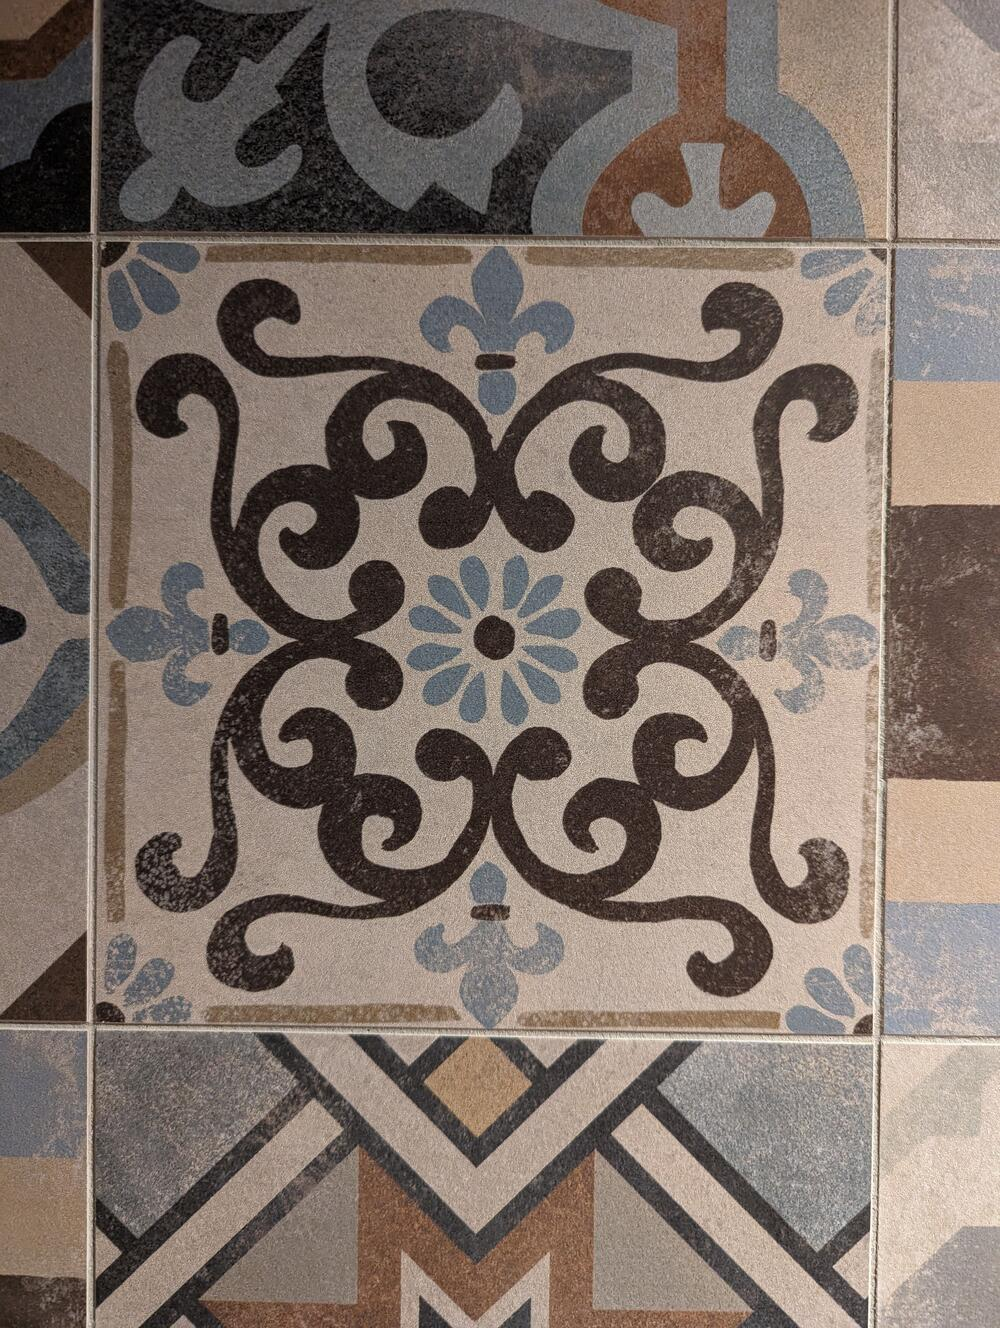
\includegraphics[height=4cm]{fliesen/fliese14.jpg} &
		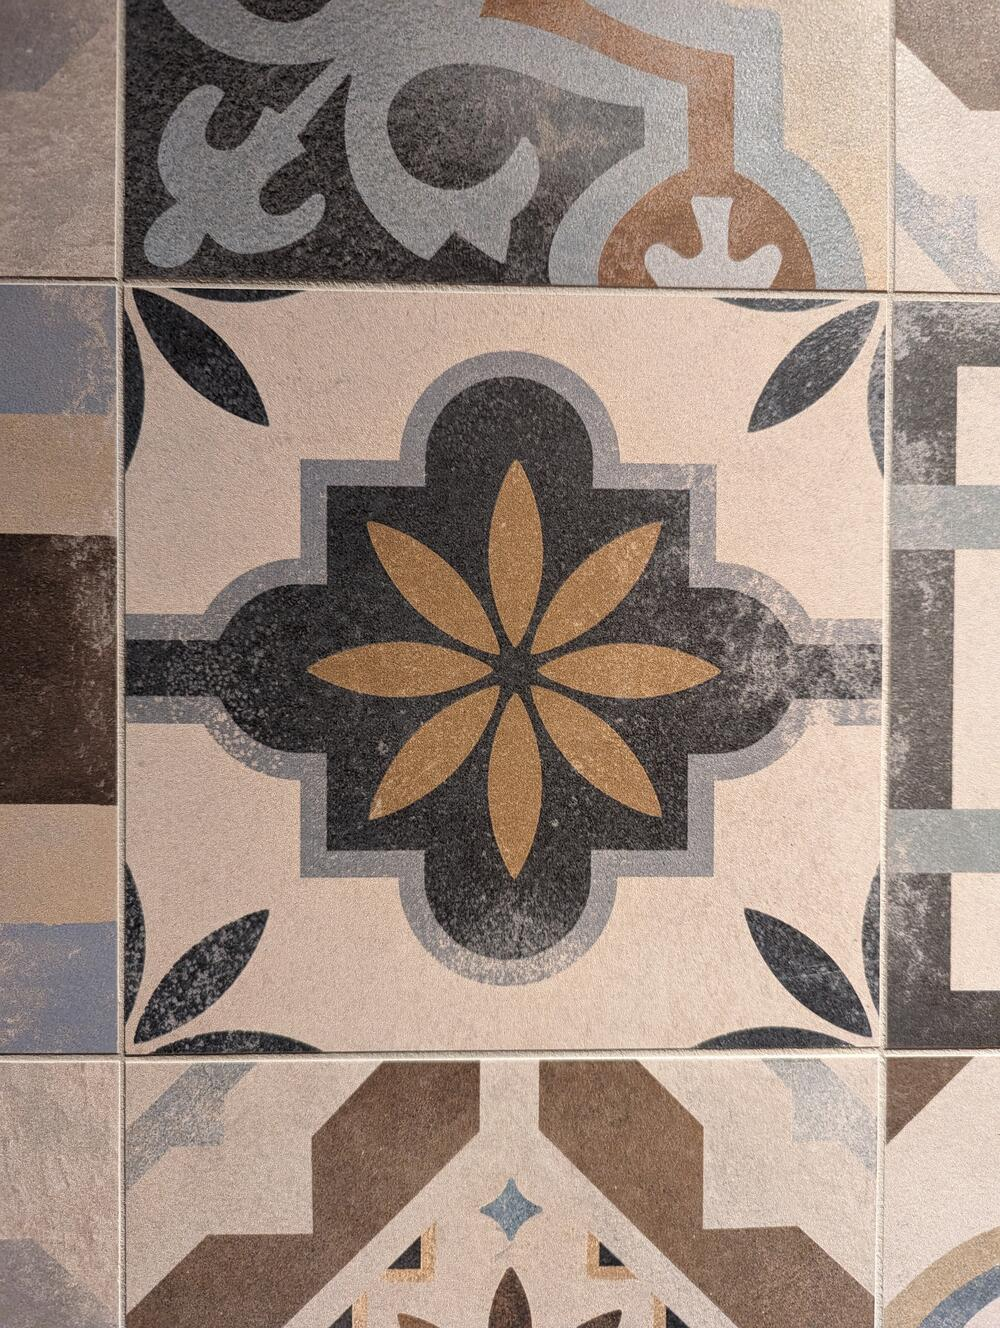
\includegraphics[height=4cm]{fliesen/fliese15.jpg} \\
		\textbf{Fliese Nr. 16} & \textbf{Fliese Nr. 17} & \textbf{Fliese Nr. 18} & \textbf{Fliese Nr. 19} & \textbf{Fliese Nr. 20} \\
		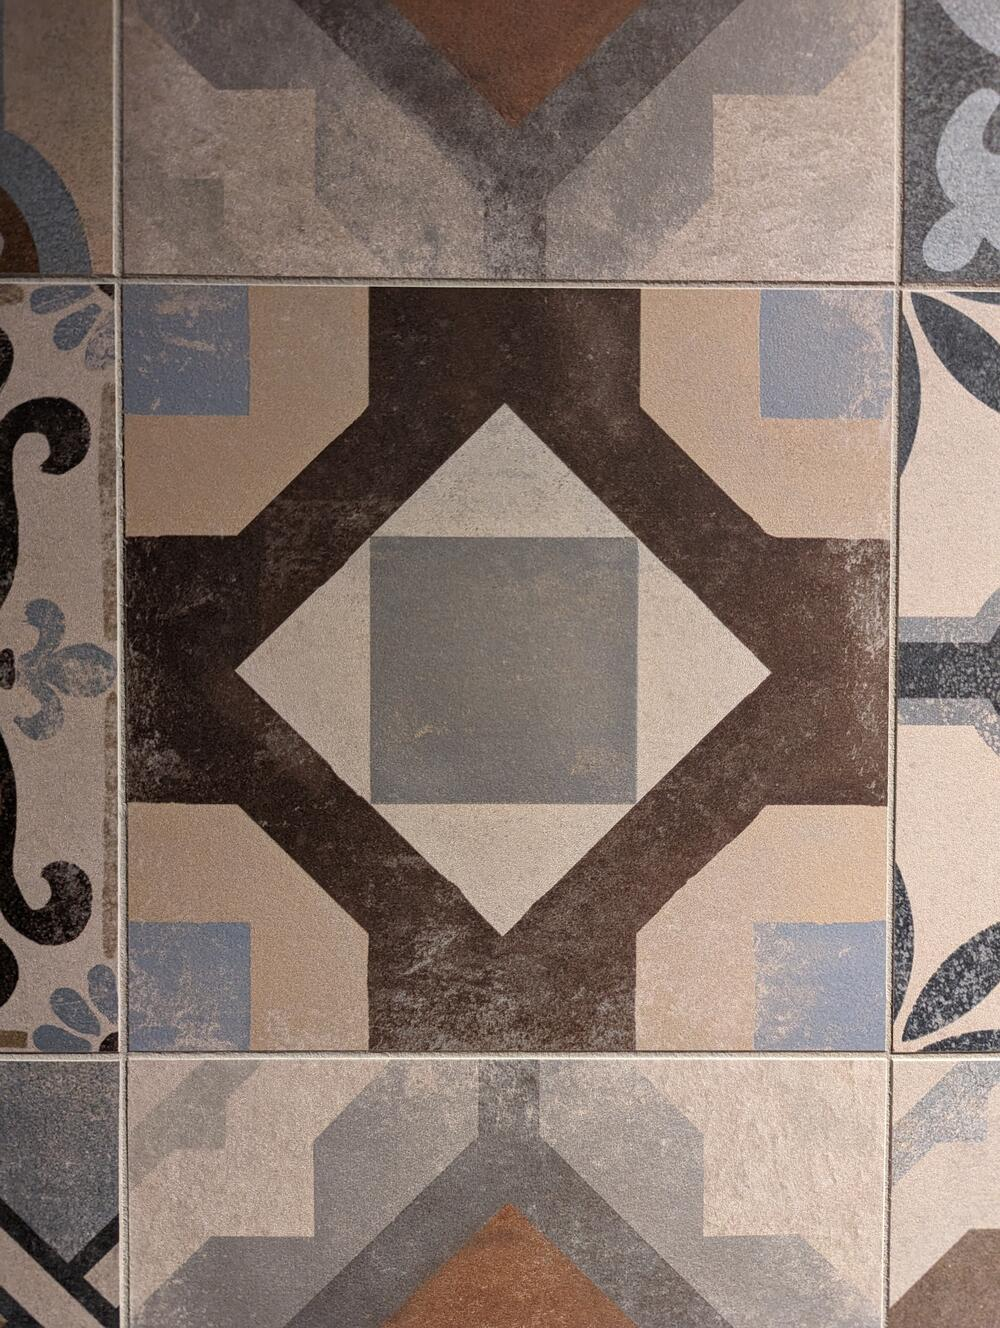
\includegraphics[height=4cm]{fliesen/fliese16.jpg} &
		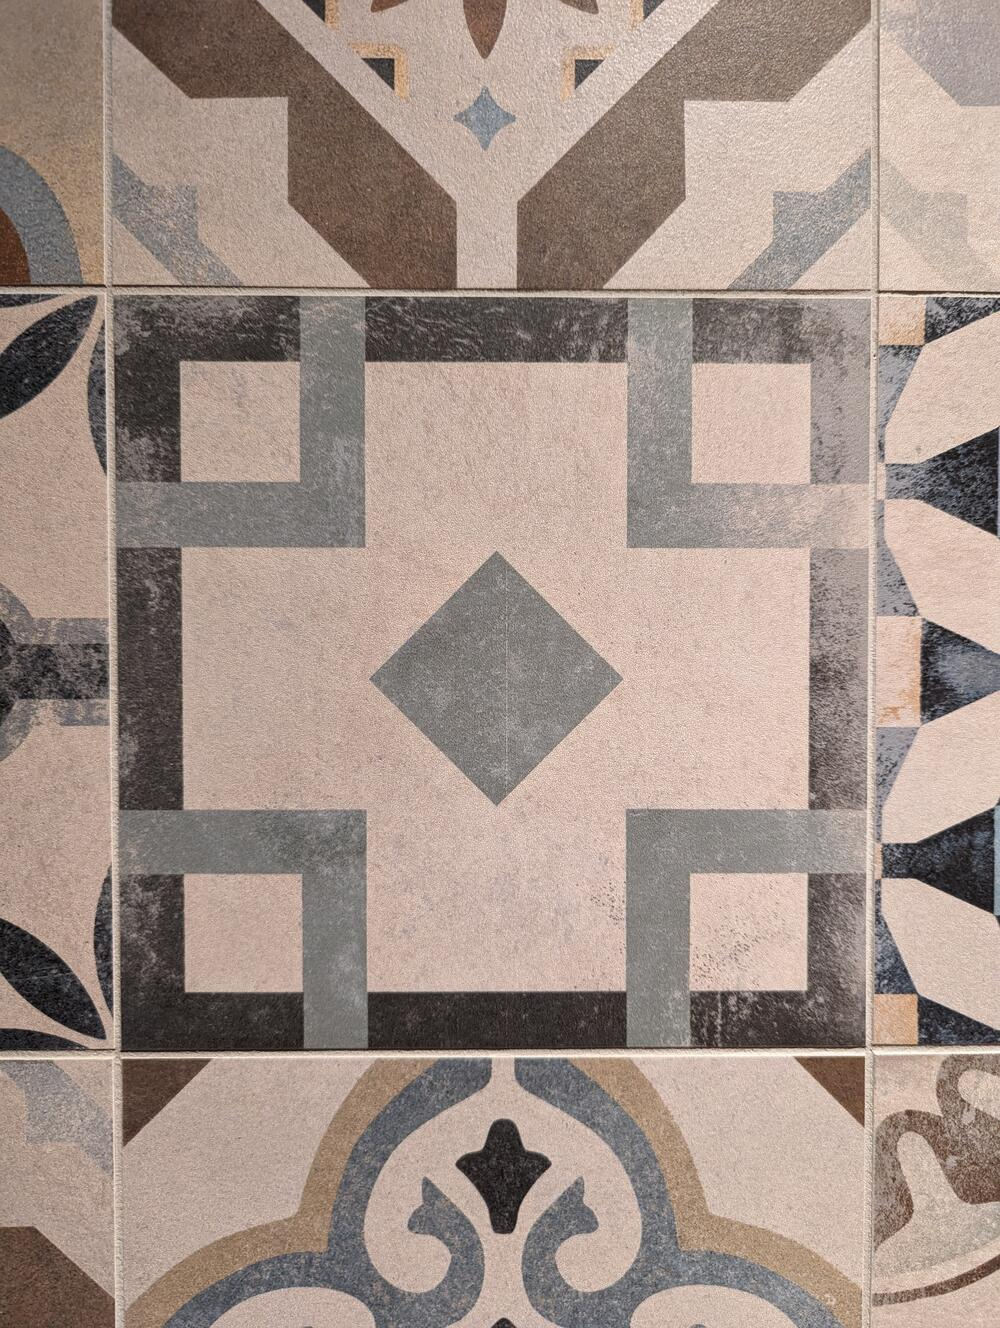
\includegraphics[height=4cm]{fliesen/fliese17.jpg} &
		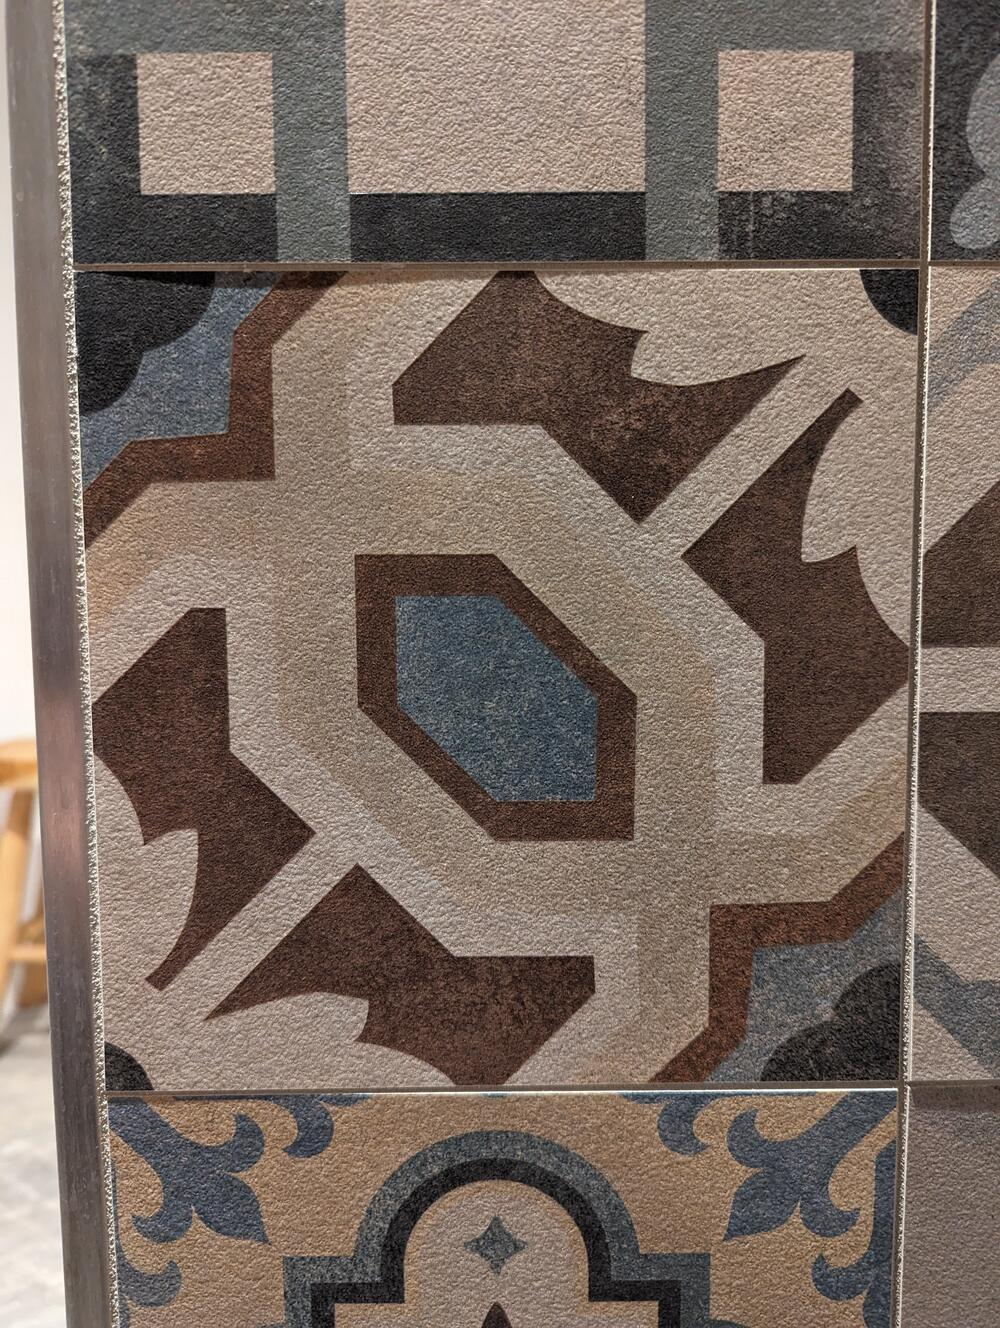
\includegraphics[height=4cm]{fliesen/fliese18.jpg} &
		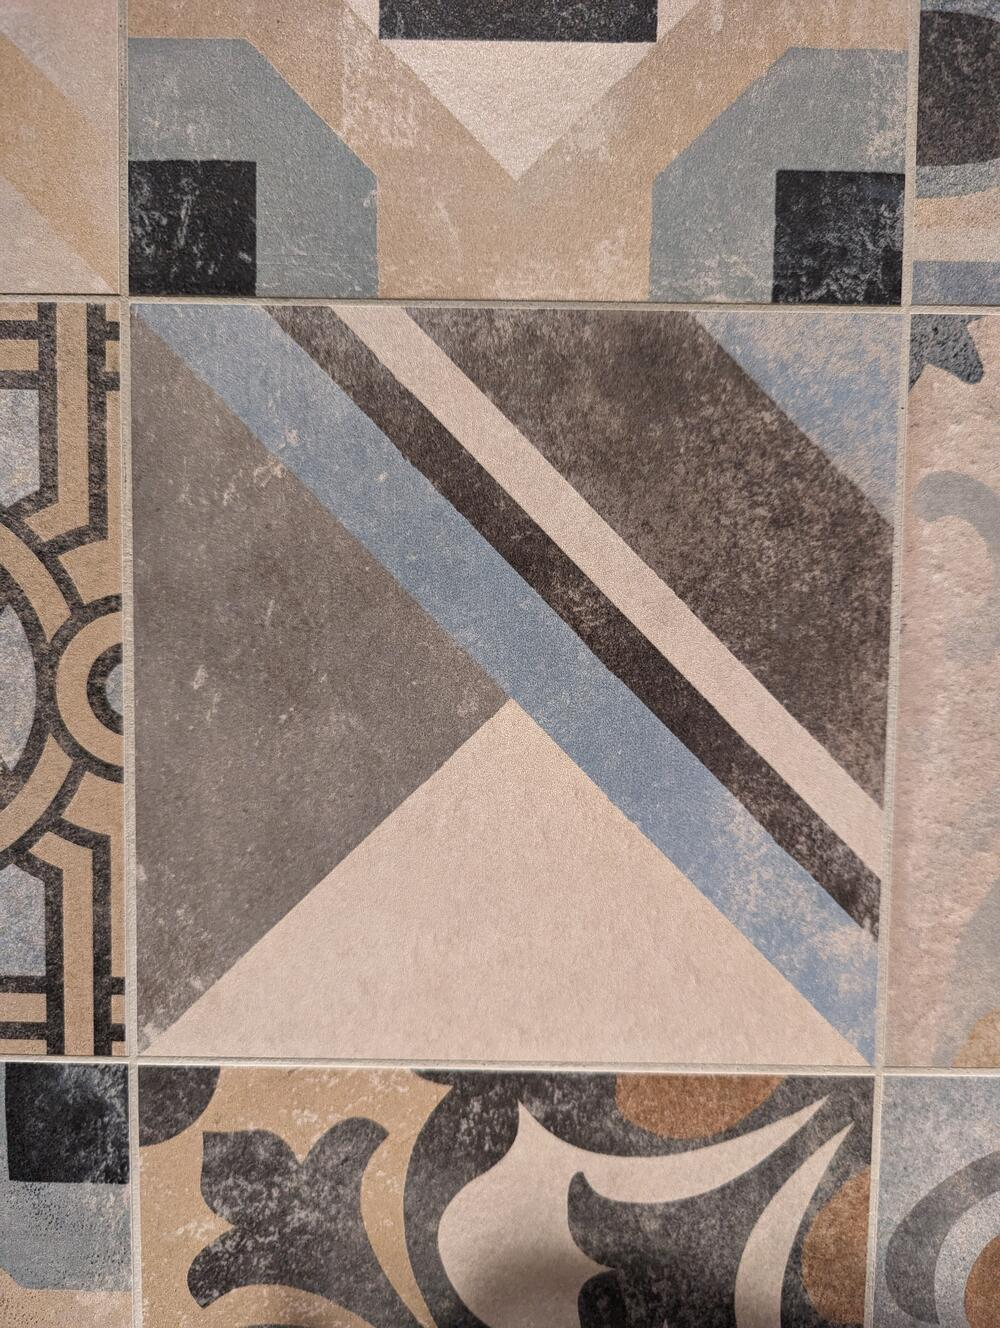
\includegraphics[height=4cm]{fliesen/fliese19.jpg} &
		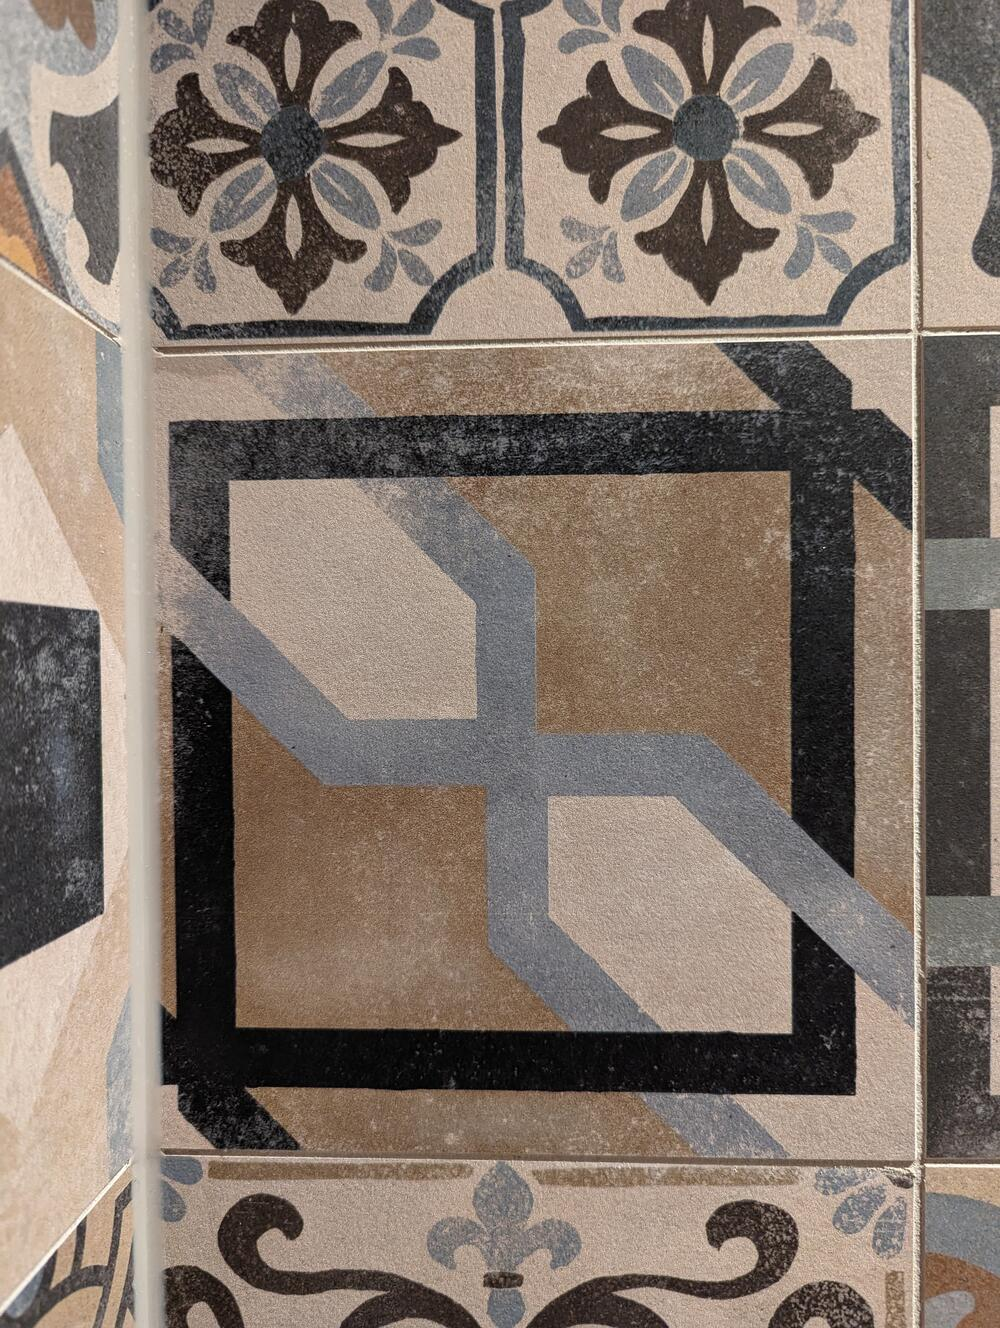
\includegraphics[height=4cm]{fliesen/fliese20.jpg} \\
	\end{tabular}
\end{figure}


\end{document}
